\hsection{Bounds of the Objective Function}%
\label{sec:objectiveFunctionBound}%
%
If we apply a heuristic algorithm, then we do not have the guarantee that the solution we get is optimal.
Usually, we do not even know if the best solution we currently have is optimal or not.
The most basic mistake that we can read in papers on optimization again and again is this:
The claim that a metaheuristic returns optimal solutions (without further proof or considerations such as those below).
It does not.
None of them do.
They can return good solutions, maybe better solutions than what we can get with any other algorithm within acceptable runtime.
But we usually do not know if a solution is optimal or not.

Well.
Usually.
But not always.

In some cases, we be able to compute a \emph{lower bound}~$\lowerBoundOf{\objf}$ for the objective function.%
%
\hsection{Definitions}%
%
\begin{definition}[Lower Bound]%
\label{def:lowerBound}%
The \emph{lower bound}~\lowerBoundOf{f} of a function~$f$ is a value such that $f(x)\geq\lowerBoundOf{f}\forall x$.%
\end{definition}%
%
We know that it is not possible that any solution can have a quality better than~$\lowerBoundOf{\objf}$.
If a solution~$\solspel\in\solutionSpace$ exists with $\objfOf{\solspel}=\lowerBoundOf{\objf}$, then this solution must be a global optimum, i.e., it is actually~\globalOptimumOf{\solspel}.

However, notice the \inQuotes{$\geq$} in \autoref{def:lowerBound}.
It means that maybe no solution exists that has this objective value.
In this case, the objective value~\objfOf{\globalOptimumOf{\solspel}} of the global optimum~\globalOptimumOf{\solspel} would actually be larger, i.e., $\objfOf{\globalOptimumOf{\solspel}}>\lowerBoundOf{\objf}$.

Having a lower bound of the objective function therefore is not directly useful for solving the problem itself.
Still, it can at least help us to understand whether our method for solving the problem is good.
For instance, if we have developed an algorithm for approximately solving a given problem and the qualities of the solutions we get are close to the lower bound, then we know that our algorithm is good.
If we even find a solution whose quality equals the lower bound, then we %
\begin{enumerate*}%
\item know that it is optimal and %
\item can stop our algorithm immediately, as we cannot further improve on this.%
\end{enumerate*}

If we get close to the lower bound, then we know that improving the result quality of the algorithm may be hard, maybe even impossible, and probably not worthwhile.
However, if we cannot produce solutions as good as or close to the lower quality bound, this does not necessarily mean that our algorithm is bad.

It should be noted that it is \emph{not} necessary to know the bounds of objective values.
Lower bounds are a \emph{\inQuotes{nice to have}} feature allowing us to better understand the performance of our algorithms.%
%
\endhsection%
%
\hsection{A Programmer's Perspective}%
%
In \autoref{lst:Objective}, we presented the API for implementing objective functions.
We extend this API by a function \codeil{lower_bound()} that can return a lower bound or~$-\infty$ if no bound is known.
(Indeed, $-\infty$ is also a valid lower bound that fulfills \autoref{def:lowerBound}.)
Furthermore, our experiment \href{\moptipyExecution}{execution API} will automatically stop the optimization processes if a solution~$\globalOptimumOf{\solspel}$ with~$\objfOf{\globalOptimumOf{\solspel}}=\lowerBoundOf{\objf}$ is reached.%
\endhsection%
%
\hsection{Example: Job Shop Scheduling}%
\label{sec:jssp:lowerBounds}%
We have already defined our solution space~$\solutionSpace$ for the \gls{JSSP} in \autoref{lst:jssp_gantt} and the objective function~$\objf$ in \autoref{lst:jssp_makespan}.
A Gantt chart with the shortest possible makespan is then a global optimum.
There may be multiple globally optimal solutions, which then would all have the same makespan.

When facing a \gls{JSSP} instance~$\instance$, we do not know whether a given Gantt chart is the globally optimal solution or not, because we do not know the shortest possible makespan.
There is no direct way in which we can compute this optimal makespan.
Actually, if we could, we would probably have solved the problem already.
However, we can, at least, compute some \emph{lower bound}~\lowerBoundOf{\objf} for the best possible makespan.

A trivial lower bound for the makespan is always 0~time units.
No schedule can complete faster than that.
Of course, this would also be a useless lower bound, because it does not tell us anything.
%
\ruleOfThumb{lowerBoundObjective}{A lower bound~\lowerBoundOf{\objf} of the objective function~\objf\ is the better and the more useful, the higher it is.}%
%
The highest possible lower bound for the quality of an optimal solution would be exactly that quality itself (because otherwise it would violate \autoref{def:lowerBound}).
As said, we are not able to build such a bound for the \gls{JSSP}.
But we can do other things.

For instance, we know that a job~\jsspJobIndex\ needs at least as long to complete as the sum~$\sum_{\jsspMachineIndex=0}^{\jsspMachines-1} \jsspOperationTime{\jsspJobIndex}{\jsspMachineIndex}$ over the processing times of all of its operations.
Imagine that we have two machines.
If there is one job whose first operation needs 20~time units on the first machine and its second operation needs 30~time units on the second machine, then we can never complete this \gls{JSSP} in less than $20+30=50$ time units.
It is also clear that no schedule can complete faster then the longest job.
Even if the other jobs in this example would need less than 50~time units in total, we still need need at least 50~time units.
So we already have one lower limit.

Furthermore, we know that the makespan of the optimal schedule also cannot be shorter than the latest \inQuotes{finishing time} of any machine~$\jsspMachineIndex$.
This finishing time is at least as big as the sum~$\jsspMachineRuntime{\jsspMachineIndex}$ of the runtimes of all the operations for this machine.
If we have two jobs, and one operation of the first job needs 30~time units on the first machine and some operation of the second job needs 60~time units on the first machine, then we will need at least $30+60=90$~time units to complete the schedule.

We can actually further refine this idea:
Each machine may have some least initial idle time~\jsspMachineStartIdle{\jsspMachineIndex}:
If the operations for machine~\jsspMachineIndex\ never come first in their job, then for each job, we need to sum up the runtimes of the operations coming \emph{before} the one on machine~$\jsspMachineIndex$.
The least initial idle time~\jsspMachineStartIdle{\jsspMachineIndex} is then the smallest of these sums.
This may be~0, if there is at least one job that \emph{first} goes to the machine, or greater than zero if no such job exists.

Similarly, each machine has a least idle time~\jsspMachineEndIdle{\jsspMachineIndex} at the end.
This is greater than zero if there is no job whose \emph{last} operation is on the machine.
Then, whenever the last job assigned to the machine has been processed by it, it still needs to go to go elsewhere and the machine must always remain idle for some time at the end of the schedule.
As lower bound for the fastest schedule that could theoretically exist, we therefore get:%
%
\begin{align}%
\lowerBoundOf{\objf} = \max\left\{\max_{\jsspJobIndex}\left\{ \sum_{\jsspMachineIndex=0}^{\jsspMachines-1} \jsspOperationTime{\jsspJobIndex}{\jsspMachineIndex}\right\} \;,\; \max_{\jsspMachineIndex} \left\{ \jsspMachineStartIdle{\jsspMachineIndex}+\jsspMachineRuntime{\jsspMachineIndex} +\jsspMachineEndIdle{\jsspMachineIndex}\right\}\right\}%
\label{eq:jsspLowerBound}%
\end{align}%
%
\autoref{eq:jsspLowerBound} is implemented in \autoref{lst:jssp_makespan_lb}, following the ideas from~\cite{T1993BFBSP}.%
%
\moptipyCode{moptipy/examples/jssp/instance.py}{--labels lb --args comments}{jssp_makespan_lb}{An implementation of \citeauthor{T1993BFBSP}'s algorithm~\cite{T1993BFBSP} represented in \autoref{eq:jsspLowerBound} to compute the lower bound of the makespan of a \gls{JSSP} instance.}%
%
\begin{figure}%
\centering%
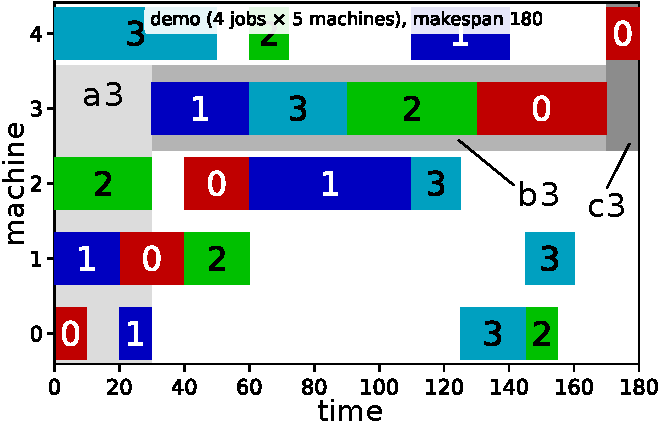
\includegraphics[width=0.55\linewidth]{\currentDir/gantt_demo_opt_with_makespan_and_lb.pdf}%
\caption{A globally optimal solution of the \instStyle{demo} instance \autoref{fig:jssp_demo_instance}, whose makespan happens to be the same as the lower bound from \autoref{eq:jsspLowerBound}.}%
\label{fig:gantt_demo_opt_with_makespan_and_lb}%
\end{figure}%

\autoref{fig:gantt_demo_opt_with_makespan_and_lb} again illustrates the globally optimal solution for our small \instStyle{demo} \gls{JSSP} instance already shown in \autoref{fig:gantt_demo_opt_with_makespan}.
Here we were lucky:
The objective value of this solution happens to be the same as the lower bound for the makespan.
Upon closer inspection, the limiting machine is the one at index~3.

We will find this by again looking at \autoref{fig:jssp_demo_instance}.
Regardless with which job we would start here, it would need to initially wait at least~$\jsspMachineStartIdle{3}=30$ time units.
The reason is that not a single first operation of any job starts at machine~3.
Every job starts at another machine.
So machine~3 can never begin its work at time index~0, since every job first needs to be processed by at least one other machine before getting to machine~3.
Job~0 would get to machine~3 the earliest after 50~time units, job~1 after~30, job~2 after~62, and job~3 after again 50~time units.
From all of these values, only the smallest one is relevant, which here is $\jsspMachineStartIdle{3}=30$~time units.

No job in the \instStyle{demo} instance finishes at machine~3 either.
This means that even if machine~3 finishes has completed all of its work, there definitely will be some operations that still need to be processed on another machine.
Job~0, for instance, needs to be processed by machine~4 for 10~time units after it has passed through machine~3.
So regardless when machine~3 finishes, the schedule will need at least 10~additional time units.
Job~1 requires 80~more time units after finishing at machine~3, job~2 also 10~time units, and job~3 again~50 time units.
From these values, again, the only smallest one is relevant, namely $\jsspMachineEndIdle{3}=10$~time units.
In other words, machine~3 needs to wait at least 30~time units before it can commence its work and will remain idle for at least 10~time units after processing the last operation.

In between, it will need to work for exactly $\jsspMachineRuntime{3}=140$~time units, the total sum of the running time of all operations assigned to it.
This means that no schedule can complete faster than $\jsspMachineFinish{3}=\jsspMachineStartIdle{3}+\jsspMachineRuntime{3}+\jsspMachineEndIdle{3}=30+140+10=180$~time units.
Thus, \autoref{fig:gantt_demo_opt_with_makespan_and_lb} illustrates the optimal solution for the \instStyle{demo} instance (and the lower bound).

Interestingly, while the last job in \autoref{fig:gantt_demo_opt_with_makespan_and_lb} is on machine~4, machine~4 does not limit us.
We could start by putting job~3 first on machine~4, so this machine could theoretically begin its work immediately at time unit~0.
Also, we could finish both job~0 and job~1 at machine~4, so there also would not necessarily be an idle time at the end of the schedule on machine~4.
Both of these facts can be seen in \autoref{fig:gantt_demo_opt_with_makespan_and_lb}.
If we could schedule all jobs on machine~4 without delay, then we would need $50+12+30+10=102$~time units.
Without starting delay and and ending idle time, this machine would limit schedules to not be shorter than 102~time units.
Since we know that machine~3 imposes a makespan no less than 180~time units, machine~4 has no impact on the lower bound of the makespan.%
%
\begin{table}%
\centering%
\caption{The lower bounds~\lowerBoundOf{\objf} for the makespan of the optimal solutions for our example problems. %
For some instances, research literature~\cite{W2019JRDAIOTJSSP} (last column) provides better (i.e., higher) lower bounds~$\lowerBoundOf{\objf}^{\star}$ than our algorithm in \autoref{lst:jssp_makespan_lb}.}%
\label{tbl:jsspLowerBoundsTable}%
%
\begin{booktabular}{lrrrll}%
name&\jsspJobs&\jsspMachines&\lowerBoundOf{\objf}&$\lowerBoundOf{\objf}^{\star}$&source for~$\lowerBoundOf{\objf}^{\star}$\\%
\midrule%
\instStyle{demo}&5&4&180&180&\autoref{eq:jsspLowerBound}\\%
\textbf{\instStyle{abz8}}&20&15&566&648&\cite{VLS2015FDSFCBS}\\%
\textbf{\instStyle{dmu67}}&40&20&5454&5589&\cite{GL2010ETSMBRSFTJSSP}\\%
\textbf{\instStyle{dmu72}}&50&15&6216&6395&\cite{GL2010ETSMBRSFTJSSP}\\%
\instStyle{la38}&15&15&943&1196&\cite{VAL1996JSSBLS}\\%
\instStyle{orb06}&10&10&930&1010&\cite{JM1999DJSSPPAF}\\%
\instStyle{swv14}&50&10&2968&2968&\autoref{eq:jsspLowerBound}\\%
\instStyle{ta65}&50&20&2725&2725&\autoref{eq:jsspLowerBound}\\%
\instStyle{ta79}&100&20&5358&5358&\autoref{eq:jsspLowerBound}\\%
\textbf{\instStyle{yn4}}&20&20&818&929&\cite{VLS2015FDSFCBS}\\%
\end{booktabular}%
\end{table}

The lower bounds for the makespans of our example problems are listed in \autoref{tbl:jsspLowerBoundsTable}.
At the time of this writing, there are four instances (\instStyle{abz8}, \instStyle{dmu67}, \instStyle{dmu72}, and \instStyle{yn4}) in our benchmark set for which no solutions have been found yet whose makespan equals the best available lower bound.
This either means that these four problems have not yet been solved to optimality or that their optimal solution has already been found but has a makespan worse than the lower bound.
In the table, we also provide better, i.e., higher lower bounds~$\lowerBoundOf{\objf}^{\star}$ that are available for some instances.
We took these from our meta-study~\cite{W2019JRDAIOTJSSP}, which aggregates many results from different papers and existing studies.
%
\endhsection%
%
\hsection{Summary}%
Now, we do not know whether it is actually possible to find a schedule whose makespan equals the lower bound.
There may simply not be any way to arrange the jobs such that no operation stalls any other operation too much.
This is why the value~\lowerBoundOf{\objf} is called lower bound:
We know no solution can be better than this, but we do not know whether a solution with such minimal makespan exists.
However, if our algorithms produce solutions with a quality close to~\lowerBoundOf{\objf}, we know that we are doing well.
Also, if we would actually find a solution with that makespan, then we would know that we have perfectly solved the problem.
\endhsection%
\endhsection%
%
